% ps2-search.tex
\documentclass{article} %The basic layout of the output document, sets things like pagesize and defaults
\usepackage{amsmath} %a package for good looking equations and symbols
\usepackage{algorithm2e} %a package for typesetting algorithms
\usepackage{caption} %a package for more complex captions for figures/tables/images
\usepackage{subcaption} %extension of the caption package
\usepackage{url} %embedded, clickable links
\usepackage{fullpage} %including this package changes the default margins to use more of the page
\usepackage{graphicx} %package for inline images
\usepackage[usenames]{xcolor} %for adding color text
\usepackage{enumitem} %for nested numbered lists (like in the questions section)

%note that the title and date are specified /before/ the "\begin{document}" command.
\title{Introduction to Artificial Intelligence\\ %double backslash (ie, "\\") are typically used to force a newline in most environments
Problem Set 2 --- Search}
\date{} %an empty string "{}" is OK here, but some environments/commands will throw an error.
\author{}

\begin{document}
\maketitle %The "\maketitle command" is what actually formats and inserts this information into the text.

%some latex magic that creates a new command for use in this document. This particular command is handy for annotating
%changes or temporary text.
\newcommand{\bphnote}[1]{\textit{\textcolor{red}{#1}}}


\section*{Instructions} %Sections and subsections create headers and are automatically numbered
In this second problem set we're going to apply a few of the search techniques we discuss in class by hand on a small toy problem, and discuss heuristics and search problem design. These questions are typically longer than what I would expect you to be able to complete in one class period, but they should serve as good practice for exams and indicate the level of understanding I am expecting. Remember, if you run into difficulties, do
\begin{itemize}
	\item Bring your questions to class and to office hours. Don't wait until you get stuck on a complicated part of a homework somewhere down the line.
	\item Attempt to complete as much as you can, and
	\item \textcolor{red}{\textbf{TURN IN YOUR WORK before the due date}}. You won't be penalized for incomplete work, or for errors in your code or logic, but you won't get any credit if you don't turn anything in. This is true for all problem set assignments in this course.
\end{itemize}

\section*{Questions}
Use the graph given in figure \ref{graph-fig} for the next few questions. Nodes are labeled with their names, edges with their weights. The starting state is ``A'' and the goal state is ``F''. When describing actions, use the notation ``A->C'' to refer to ``moving from state A to state C'', which in this graph has a cost of 6. Use alphabetical order in the case of ties.

\begin{figure}
\begin{center}
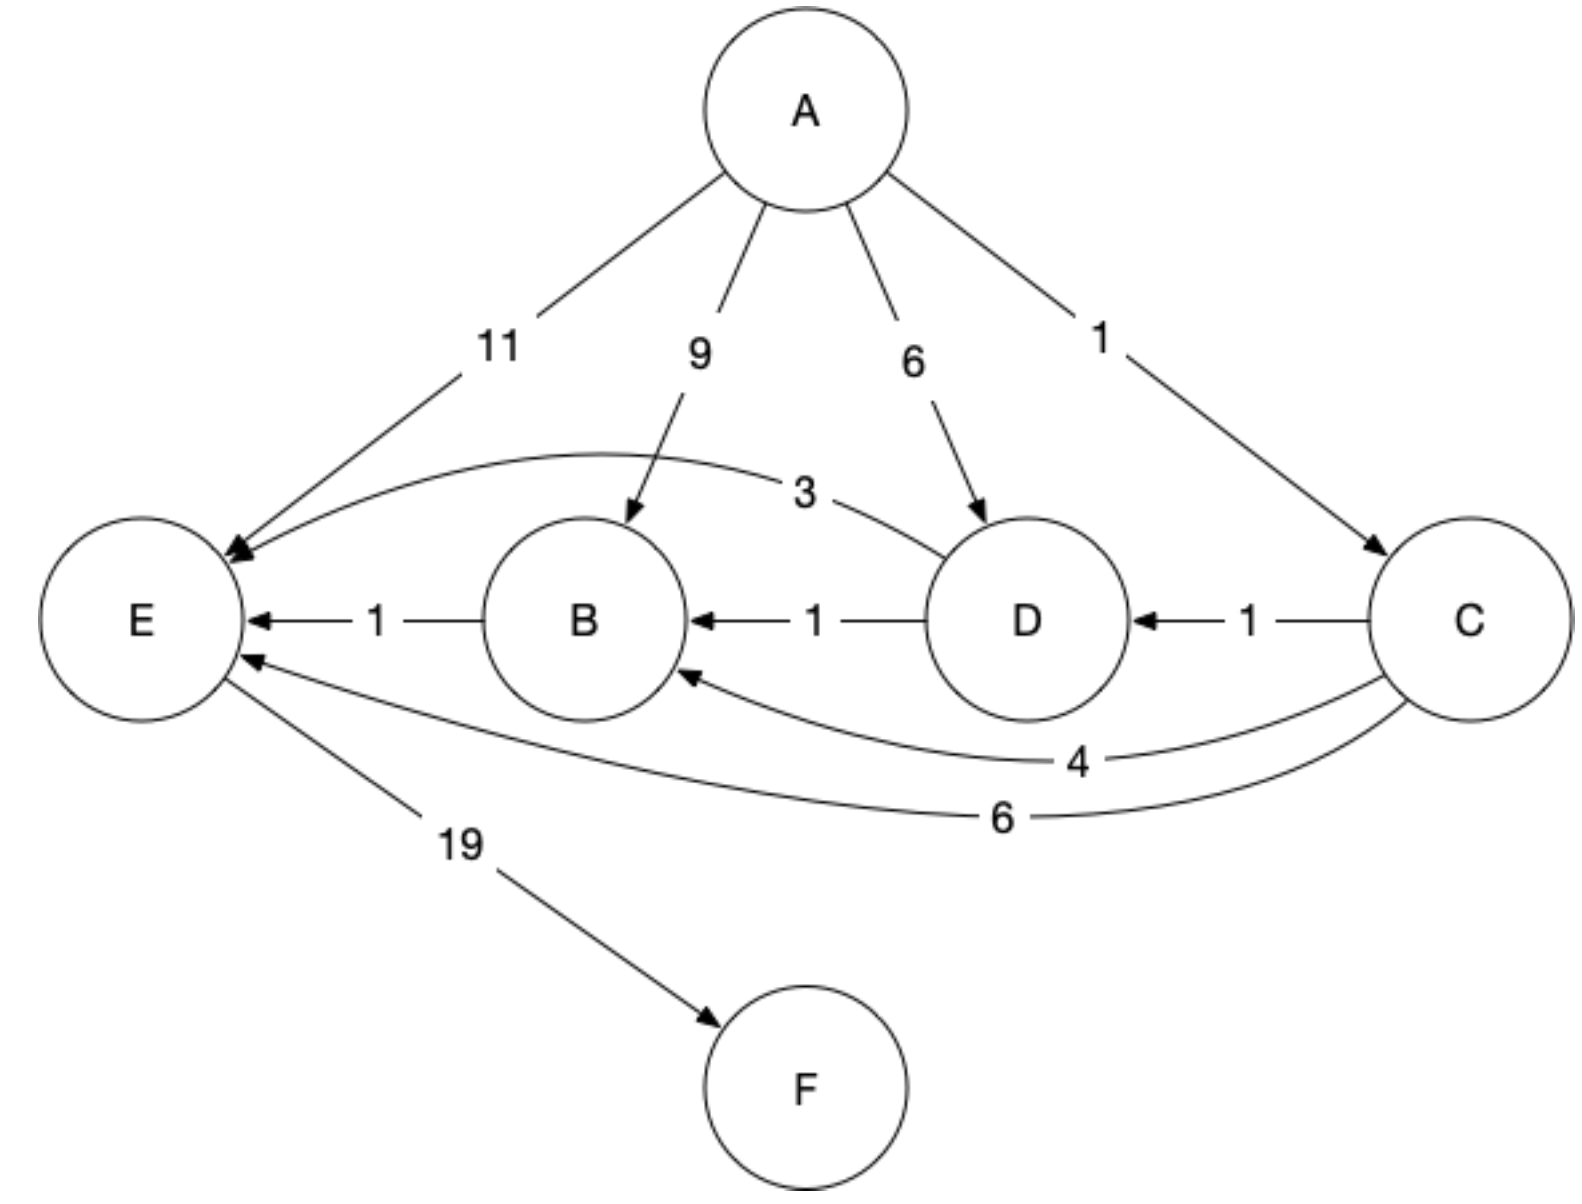
\includegraphics[height=0.3\textheight]{graph-fig}
\caption{A small state-space graph.}
\label{graph-fig}
\end{center}
\end{figure}

\begin{figure}
\begin{center}
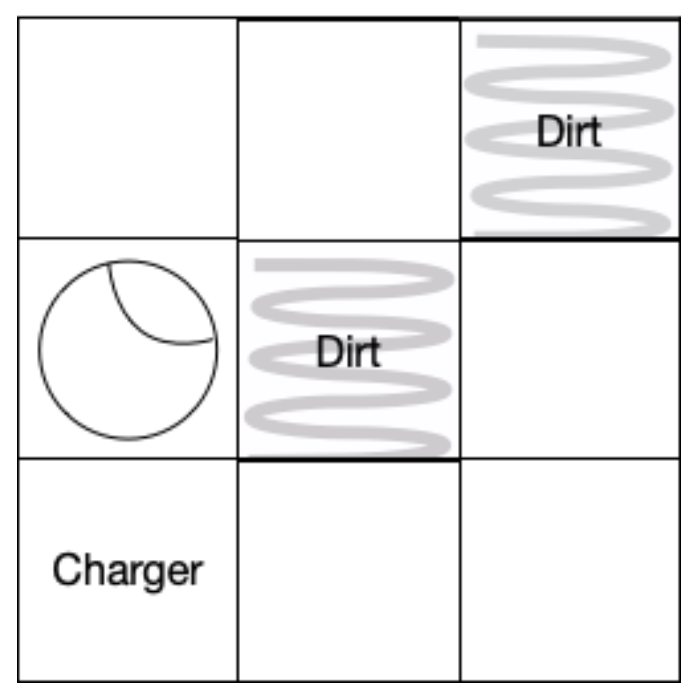
\includegraphics[height=0.3\textheight]{roomba-world}
\caption{A small roomba world.}
\label{roomba-world}
\end{center}
\end{figure}


\begin{enumerate}
	\item Find a path from the start (A) to the goal (F) using the \textbf{Depth First Search} version of the \textbf{Generic Search Algorithm} discussed in class, making sure to
	\begin{enumerate}
		\item Show the status of the open and closed data structures for each iteration.
		\item Show the final search tree after the goal state is reached.
		\item Show the final result (path).
	\end{enumerate}
	\item Answer the same three questions for the Uniform Cost Search version.
	\item Answer the same three questions for \(\textrm{A}^*\) search using the following heuristic: \begin{tabular}{c|c}State & \(h(\textrm{State})\)\\ \hline A & 23\\ B& 3\\ C& 13\\ D& 7\\ E& 0\\ F&0\end{tabular}
	\item Is this heuristic \textbf{admissible}? Explain why or why not.
	\item This graph is part of a family of similar graphs known as Martelli's family that is specifically designed to illustrate why \textbf{consistency} is important for a heuristic. Replace the heuristic function from question 3 with one that is consistent and re-do the search. How was the search different?
	\item Our friendly vacuum robot needs to clean the room illustrated in figure \ref{roomba-world}. For the purposes of this example, the vacuum is running the entire time, so the only actions are to move between adjacent cells. The robot's goal is to visit each of the spaces with dirt, and return to its charger afterwards. Define this task as a search problem and give \textbf{all} the components necessary to solve it using either uninformed or informed search.
	\item Given your problem definition, which technique would you use?
	What would change if the robot had to recharge after cleaning a dirty cell? Describe in words how this would change your problem definition.

\end{enumerate}

\section*{Submission}
Write up your answers to the given questions as a single PDF file. You can use whatever text editor you prefer (or even write out your solution by hand and scan the result), but remember to export as (or print to) PDF, non-PDF files aren't allowed. If you're feeling ambitious, \LaTeX produces high-quality PDF files, and is the format of choice for research papers written across computer science disciplines. This document was produced using \LaTeX: the zip file it came in includes the source with helpful examples and you are welcome to use it as a starting point for your own work.

\end{document}